% Created by tikzDevice version 0.12.6 on 2025-04-16 12:14:21
% !TEX encoding = UTF-8 Unicode
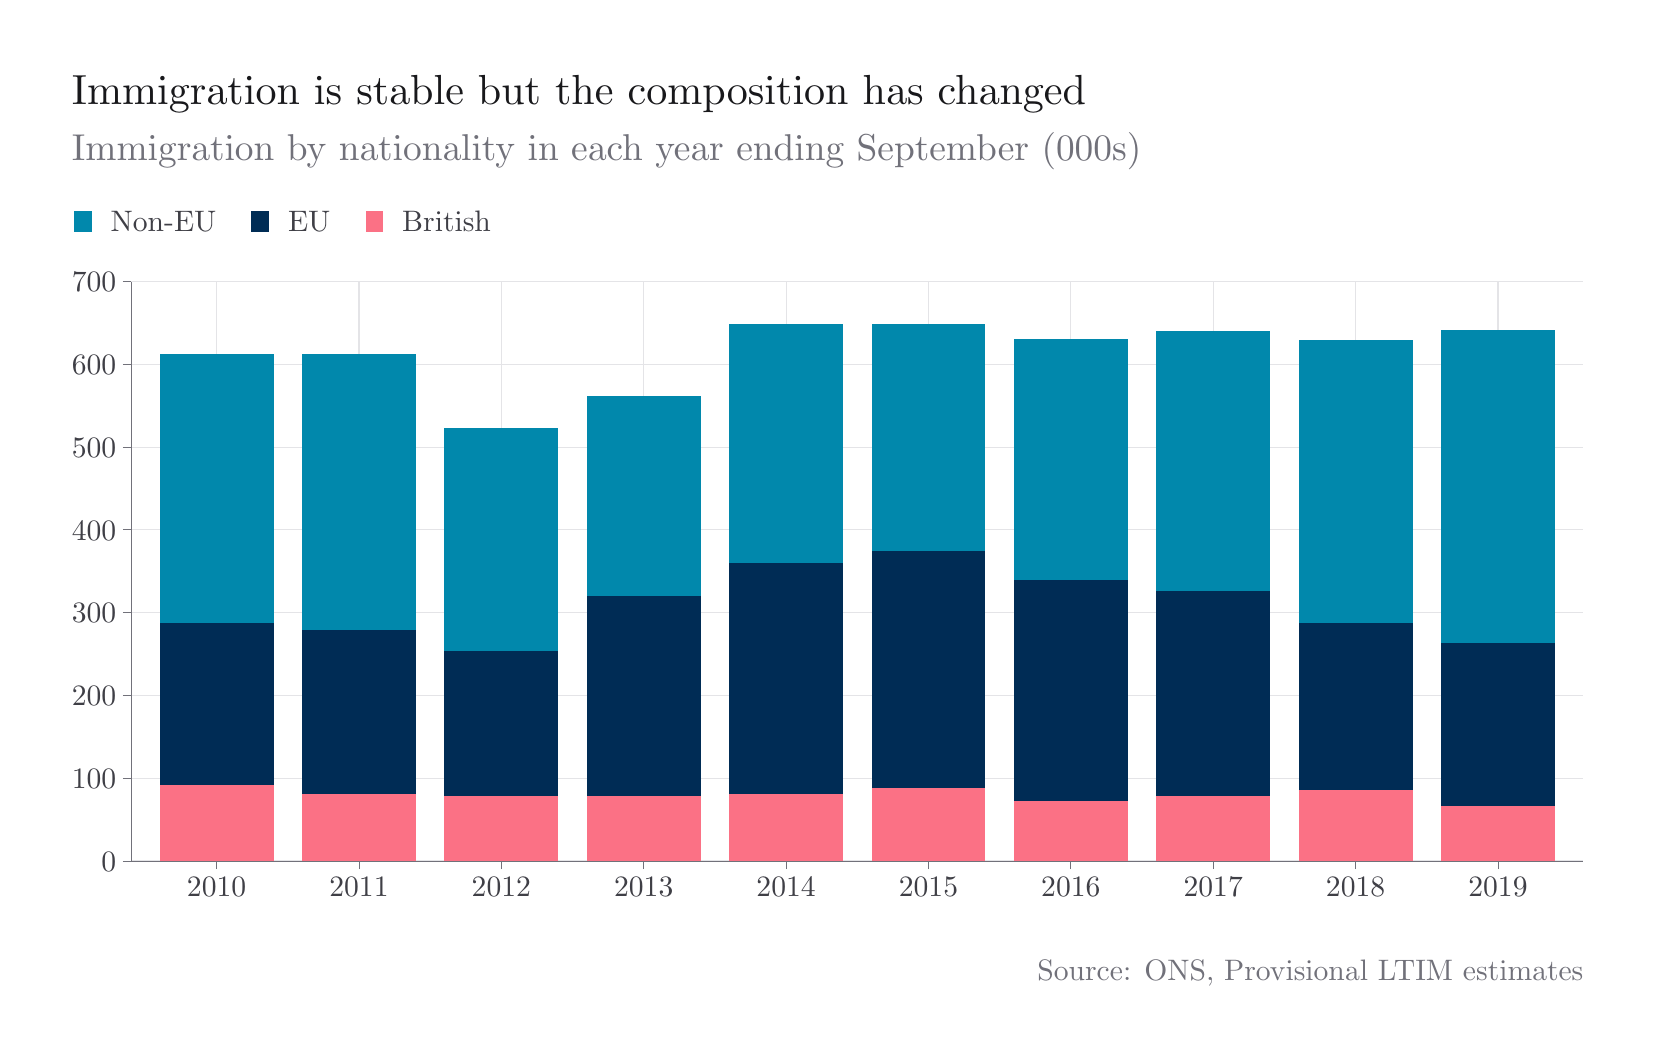
\begin{tikzpicture}[x=1pt,y=1pt]
\definecolor{fillColor}{RGB}{255,255,255}
\path[use as bounding box,fill=fillColor] (0,0) rectangle (578.16,361.35);
\begin{scope}
\path[clip] (  0.00,  0.00) rectangle (578.16,361.35);
\definecolor{drawColor}{RGB}{255,255,255}

\path[draw=drawColor,line width= 0.6pt,line join=round,line cap=round,fill=fillColor] (  0.00,  0.00) rectangle (578.16,361.35);
\end{scope}
\begin{scope}
\path[clip] ( 37.40, 60.25) rectangle (562.16,269.59);
\definecolor{drawColor}{RGB}{255,255,255}
\definecolor{fillColor}{RGB}{255,255,255}

\path[draw=drawColor,line width= 0.6pt,line join=round,line cap=round,fill=fillColor] ( 37.40, 60.25) rectangle (562.16,269.59);
\definecolor{drawColor}{RGB}{228,228,231}

\path[draw=drawColor,line width= 0.4pt,line join=round] ( 37.40, 60.25) --
	(562.16, 60.25);

\path[draw=drawColor,line width= 0.4pt,line join=round] ( 37.40, 90.15) --
	(562.16, 90.15);

\path[draw=drawColor,line width= 0.4pt,line join=round] ( 37.40,120.06) --
	(562.16,120.06);

\path[draw=drawColor,line width= 0.4pt,line join=round] ( 37.40,149.96) --
	(562.16,149.96);

\path[draw=drawColor,line width= 0.4pt,line join=round] ( 37.40,179.87) --
	(562.16,179.87);

\path[draw=drawColor,line width= 0.4pt,line join=round] ( 37.40,209.78) --
	(562.16,209.78);

\path[draw=drawColor,line width= 0.4pt,line join=round] ( 37.40,239.68) --
	(562.16,239.68);

\path[draw=drawColor,line width= 0.4pt,line join=round] ( 37.40,269.59) --
	(562.16,269.59);

\path[draw=drawColor,line width= 0.4pt,line join=round] ( 68.27, 60.25) --
	( 68.27,269.59);

\path[draw=drawColor,line width= 0.4pt,line join=round] (119.72, 60.25) --
	(119.72,269.59);

\path[draw=drawColor,line width= 0.4pt,line join=round] (171.16, 60.25) --
	(171.16,269.59);

\path[draw=drawColor,line width= 0.4pt,line join=round] (222.61, 60.25) --
	(222.61,269.59);

\path[draw=drawColor,line width= 0.4pt,line join=round] (274.06, 60.25) --
	(274.06,269.59);

\path[draw=drawColor,line width= 0.4pt,line join=round] (325.50, 60.25) --
	(325.50,269.59);

\path[draw=drawColor,line width= 0.4pt,line join=round] (376.95, 60.25) --
	(376.95,269.59);

\path[draw=drawColor,line width= 0.4pt,line join=round] (428.40, 60.25) --
	(428.40,269.59);

\path[draw=drawColor,line width= 0.4pt,line join=round] (479.84, 60.25) --
	(479.84,269.59);

\path[draw=drawColor,line width= 0.4pt,line join=round] (531.29, 60.25) --
	(531.29,269.59);
\definecolor{fillColor}{RGB}{251,113,133}

\path[fill=fillColor] ( 47.69, 60.25) rectangle ( 88.85, 87.76);

\path[fill=fillColor] ( 99.14, 60.25) rectangle (140.30, 84.47);

\path[fill=fillColor] (150.58, 60.25) rectangle (191.74, 83.87);

\path[fill=fillColor] (202.03, 60.25) rectangle (243.19, 83.87);

\path[fill=fillColor] (253.48, 60.25) rectangle (294.64, 84.47);

\path[fill=fillColor] (304.93, 60.25) rectangle (346.08, 86.56);

\path[fill=fillColor] (356.37, 60.25) rectangle (397.53, 81.78);

\path[fill=fillColor] (407.82, 60.25) rectangle (448.98, 83.57);

\path[fill=fillColor] (459.27, 60.25) rectangle (500.42, 85.97);

\path[fill=fillColor] (510.71, 60.25) rectangle (551.87, 80.28);
\definecolor{fillColor}{RGB}{0,44,85}

\path[fill=fillColor] ( 47.69, 87.76) rectangle ( 88.85,146.08);

\path[fill=fillColor] ( 99.14, 84.47) rectangle (140.30,143.68);

\path[fill=fillColor] (150.58, 83.87) rectangle (191.74,136.21);

\path[fill=fillColor] (202.03, 83.87) rectangle (243.19,155.95);

\path[fill=fillColor] (253.48, 84.47) rectangle (294.64,167.91);

\path[fill=fillColor] (304.93, 86.56) rectangle (346.08,172.10);

\path[fill=fillColor] (356.37, 81.78) rectangle (397.53,161.63);

\path[fill=fillColor] (407.82, 83.57) rectangle (448.98,157.74);

\path[fill=fillColor] (459.27, 85.97) rectangle (500.42,146.38);

\path[fill=fillColor] (510.71, 80.28) rectangle (551.87,138.90);
\definecolor{fillColor}{RGB}{1,136,172}

\path[fill=fillColor] ( 47.69,146.08) rectangle ( 88.85,243.57);

\path[fill=fillColor] ( 99.14,143.68) rectangle (140.30,243.57);

\path[fill=fillColor] (150.58,136.21) rectangle (191.74,216.66);

\path[fill=fillColor] (202.03,155.95) rectangle (243.19,228.32);

\path[fill=fillColor] (253.48,167.91) rectangle (294.64,254.34);

\path[fill=fillColor] (304.93,172.10) rectangle (346.08,254.34);

\path[fill=fillColor] (356.37,161.63) rectangle (397.53,248.96);

\path[fill=fillColor] (407.82,157.74) rectangle (448.98,251.65);

\path[fill=fillColor] (459.27,146.38) rectangle (500.42,248.66);

\path[fill=fillColor] (510.71,138.90) rectangle (551.87,252.24);
\end{scope}
\begin{scope}
\path[clip] (  0.00,  0.00) rectangle (578.16,361.35);
\definecolor{drawColor}{RGB}{113,113,122}

\path[draw=drawColor,line width= 0.3pt,line join=round] ( 37.40, 60.25) --
	( 37.40,269.59);
\end{scope}
\begin{scope}
\path[clip] (  0.00,  0.00) rectangle (578.16,361.35);
\definecolor{drawColor}{RGB}{63,63,70}

\node[text=drawColor,anchor=base east,inner sep=0pt, outer sep=0pt, scale=  1.07] at ( 32.00, 56.57) {0};

\node[text=drawColor,anchor=base east,inner sep=0pt, outer sep=0pt, scale=  1.07] at ( 32.00, 86.48) {100};

\node[text=drawColor,anchor=base east,inner sep=0pt, outer sep=0pt, scale=  1.07] at ( 32.00,116.38) {200};

\node[text=drawColor,anchor=base east,inner sep=0pt, outer sep=0pt, scale=  1.07] at ( 32.00,146.29) {300};

\node[text=drawColor,anchor=base east,inner sep=0pt, outer sep=0pt, scale=  1.07] at ( 32.00,176.20) {400};

\node[text=drawColor,anchor=base east,inner sep=0pt, outer sep=0pt, scale=  1.07] at ( 32.00,206.10) {500};

\node[text=drawColor,anchor=base east,inner sep=0pt, outer sep=0pt, scale=  1.07] at ( 32.00,236.01) {600};

\node[text=drawColor,anchor=base east,inner sep=0pt, outer sep=0pt, scale=  1.07] at ( 32.00,265.92) {700};
\end{scope}
\begin{scope}
\path[clip] (  0.00,  0.00) rectangle (578.16,361.35);
\definecolor{drawColor}{RGB}{113,113,122}

\path[draw=drawColor,line width= 0.3pt,line join=round] ( 34.40, 60.25) --
	( 37.40, 60.25);

\path[draw=drawColor,line width= 0.3pt,line join=round] ( 34.40, 90.15) --
	( 37.40, 90.15);

\path[draw=drawColor,line width= 0.3pt,line join=round] ( 34.40,120.06) --
	( 37.40,120.06);

\path[draw=drawColor,line width= 0.3pt,line join=round] ( 34.40,149.96) --
	( 37.40,149.96);

\path[draw=drawColor,line width= 0.3pt,line join=round] ( 34.40,179.87) --
	( 37.40,179.87);

\path[draw=drawColor,line width= 0.3pt,line join=round] ( 34.40,209.78) --
	( 37.40,209.78);

\path[draw=drawColor,line width= 0.3pt,line join=round] ( 34.40,239.68) --
	( 37.40,239.68);

\path[draw=drawColor,line width= 0.3pt,line join=round] ( 34.40,269.59) --
	( 37.40,269.59);
\end{scope}
\begin{scope}
\path[clip] (  0.00,  0.00) rectangle (578.16,361.35);
\definecolor{drawColor}{RGB}{113,113,122}

\path[draw=drawColor,line width= 0.3pt,line join=round] ( 37.40, 60.25) --
	(562.16, 60.25);
\end{scope}
\begin{scope}
\path[clip] (  0.00,  0.00) rectangle (578.16,361.35);
\definecolor{drawColor}{RGB}{113,113,122}

\path[draw=drawColor,line width= 0.3pt,line join=round] ( 68.27, 57.25) --
	( 68.27, 60.25);

\path[draw=drawColor,line width= 0.3pt,line join=round] (119.72, 57.25) --
	(119.72, 60.25);

\path[draw=drawColor,line width= 0.3pt,line join=round] (171.16, 57.25) --
	(171.16, 60.25);

\path[draw=drawColor,line width= 0.3pt,line join=round] (222.61, 57.25) --
	(222.61, 60.25);

\path[draw=drawColor,line width= 0.3pt,line join=round] (274.06, 57.25) --
	(274.06, 60.25);

\path[draw=drawColor,line width= 0.3pt,line join=round] (325.50, 57.25) --
	(325.50, 60.25);

\path[draw=drawColor,line width= 0.3pt,line join=round] (376.95, 57.25) --
	(376.95, 60.25);

\path[draw=drawColor,line width= 0.3pt,line join=round] (428.40, 57.25) --
	(428.40, 60.25);

\path[draw=drawColor,line width= 0.3pt,line join=round] (479.84, 57.25) --
	(479.84, 60.25);

\path[draw=drawColor,line width= 0.3pt,line join=round] (531.29, 57.25) --
	(531.29, 60.25);
\end{scope}
\begin{scope}
\path[clip] (  0.00,  0.00) rectangle (578.16,361.35);
\definecolor{drawColor}{RGB}{63,63,70}

\node[text=drawColor,anchor=base,inner sep=0pt, outer sep=0pt, scale=  1.07] at ( 68.27, 47.50) {2010};

\node[text=drawColor,anchor=base,inner sep=0pt, outer sep=0pt, scale=  1.07] at (119.72, 47.50) {2011};

\node[text=drawColor,anchor=base,inner sep=0pt, outer sep=0pt, scale=  1.07] at (171.16, 47.50) {2012};

\node[text=drawColor,anchor=base,inner sep=0pt, outer sep=0pt, scale=  1.07] at (222.61, 47.50) {2013};

\node[text=drawColor,anchor=base,inner sep=0pt, outer sep=0pt, scale=  1.07] at (274.06, 47.50) {2014};

\node[text=drawColor,anchor=base,inner sep=0pt, outer sep=0pt, scale=  1.07] at (325.50, 47.50) {2015};

\node[text=drawColor,anchor=base,inner sep=0pt, outer sep=0pt, scale=  1.07] at (376.95, 47.50) {2016};

\node[text=drawColor,anchor=base,inner sep=0pt, outer sep=0pt, scale=  1.07] at (428.40, 47.50) {2017};

\node[text=drawColor,anchor=base,inner sep=0pt, outer sep=0pt, scale=  1.07] at (479.84, 47.50) {2018};

\node[text=drawColor,anchor=base,inner sep=0pt, outer sep=0pt, scale=  1.07] at (531.29, 47.50) {2019};
\end{scope}
\begin{scope}
\path[clip] (  0.00,  0.00) rectangle (578.16,361.35);
\definecolor{drawColor}{RGB}{255,255,255}
\definecolor{fillColor}{RGB}{255,255,255}

\path[draw=drawColor,line width= 0.6pt,line join=round,line cap=round,fill=fillColor] ( 16.00,281.59) rectangle (167.28,296.01);
\end{scope}
\begin{scope}
\path[clip] (  0.00,  0.00) rectangle (578.16,361.35);
\definecolor{drawColor}{RGB}{255,255,255}
\definecolor{fillColor}{RGB}{255,255,255}

\path[draw=drawColor,line width= 0.6pt,line join=round,line cap=round,fill=fillColor] ( 16.00,286.59) rectangle ( 24.00,296.01);
\definecolor{fillColor}{RGB}{1,136,172}

\path[fill=fillColor] ( 16.78,287.37) rectangle ( 23.22,295.24);
\end{scope}
\begin{scope}
\path[clip] (  0.00,  0.00) rectangle (578.16,361.35);
\definecolor{drawColor}{RGB}{255,255,255}
\definecolor{fillColor}{RGB}{255,255,255}

\path[draw=drawColor,line width= 0.6pt,line join=round,line cap=round,fill=fillColor] ( 80.08,286.59) rectangle ( 88.08,296.01);
\definecolor{fillColor}{RGB}{0,44,85}

\path[fill=fillColor] ( 80.85,287.37) rectangle ( 87.30,295.24);
\end{scope}
\begin{scope}
\path[clip] (  0.00,  0.00) rectangle (578.16,361.35);
\definecolor{drawColor}{RGB}{255,255,255}
\definecolor{fillColor}{RGB}{255,255,255}

\path[draw=drawColor,line width= 0.6pt,line join=round,line cap=round,fill=fillColor] (121.34,286.59) rectangle (129.34,296.01);
\definecolor{fillColor}{RGB}{251,113,133}

\path[fill=fillColor] (122.11,287.37) rectangle (128.56,295.24);
\end{scope}
\begin{scope}
\path[clip] (  0.00,  0.00) rectangle (578.16,361.35);
\definecolor{drawColor}{RGB}{63,63,70}

\node[text=drawColor,anchor=base west,inner sep=0pt, outer sep=0pt, scale=  1.07] at ( 30.00,287.63) {Non-EU};
\end{scope}
\begin{scope}
\path[clip] (  0.00,  0.00) rectangle (578.16,361.35);
\definecolor{drawColor}{RGB}{63,63,70}

\node[text=drawColor,anchor=base west,inner sep=0pt, outer sep=0pt, scale=  1.07] at ( 94.08,287.63) {EU};
\end{scope}
\begin{scope}
\path[clip] (  0.00,  0.00) rectangle (578.16,361.35);
\definecolor{drawColor}{RGB}{63,63,70}

\node[text=drawColor,anchor=base west,inner sep=0pt, outer sep=0pt, scale=  1.07] at (135.34,287.63) {British};
\end{scope}
\begin{scope}
\path[clip] (  0.00,  0.00) rectangle (578.16,361.35);
\definecolor{drawColor}{RGB}{113,113,122}

\node[text=drawColor,anchor=base west,inner sep=0pt, outer sep=0pt, scale=  1.35] at ( 16.00,313.33) {Immigration by nationality in each year ending September (000s)};
\end{scope}
\begin{scope}
\path[clip] (  0.00,  0.00) rectangle (578.16,361.35);
\definecolor{drawColor}{RGB}{24,24,27}

\node[text=drawColor,anchor=base west,inner sep=0pt, outer sep=0pt, scale=  1.52] at ( 16.00,333.41) {Immigration is stable but the composition has changed};
\end{scope}
\begin{scope}
\path[clip] (  0.00,  0.00) rectangle (578.16,361.35);
\definecolor{drawColor}{RGB}{113,113,122}

\node[text=drawColor,anchor=base east,inner sep=0pt, outer sep=0pt, scale=  1.07] at (562.16, 17.04) {Source: ONS, Provisional LTIM estimates};
\end{scope}
\end{tikzpicture}
